\documentclass{article}
\author{
  Torrent Gorjon, Xavier\\
  \texttt{Xavier.TorrentGorjon@os3.nl}
}
\title{InterNetworking and Routing}

\usepackage{graphicx}

\usepackage[backend=bibtex]{biblatex}

\bibliography{references}


\begin{document}


\begin{titlepage}
\center
\textsc{}\\[1cm]
\textsc{\LARGE University of Amsterdam}\\[1.5cm]

\textsc{\Large InterNetworking and Routing}\\[0.5cm]

\textsc{\Large For Dummies}\\[0.5cm]


\includegraphics[scale=1]{images/uva.png}\\[3cm]


\begin{minipage}{0.4 \textwidth}
\begin{center}
Xavier Torrent Gorj\'{o}n \\[0.5cm]
\emph{Xavier.TorrentGorjon@os3.nl}\\[0.5cm]
\end{center}
\end{minipage}
\hfill\\[0.5cm]

{\large \today} 


\end{titlepage}


\newpage

\tableofcontents

\newpage

\section{Overview}


\subsection{OSI Model}

\begin{center}
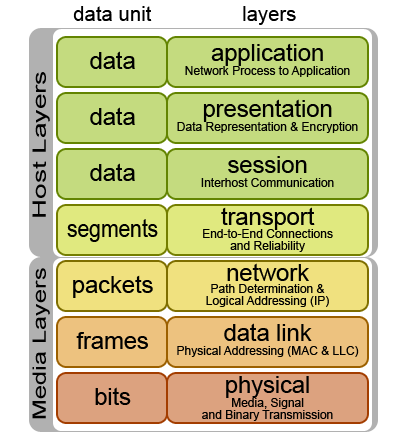
\includegraphics[scale=0.7]{images/OSI-model.png}\\[1cm]
\end{center}


\subsection{Interfaces and Protocols}

\begin{description}
	\item[Interfaces] Interfaces connect different layers on the same computer. Uses Protocol Data Units (PDU).
	\item[Protocols] Protocols are used to communicate between parties data on a specific layer. Uses Service Data Units (SDU) inside Service Access Points (SAP).
\end{description}


\subsection{Encapsulation and Multiplexing}

\begin{description}
	\item[Encapsulation] When data units go down one level in the layer model, headers are added to add information regarding the current layer.
	\item[Multiplexing] Multiple protocols can coexist on the same layer. However, when going down the layer model, these protocols should be treated equally. For example, TCP and UDP are multiplexed down at the IP level, and demultiplexed back when reading the information of IP packets.\footnote{\url{http://www.tcpipguide.com/free/t_TCPIPProcessesMultiplexingandClientServerApplicati-2.htm}}
\end{description}


\subsection{ES Models: Strong vs Weak}

\begin{description}
	\item[Strong ES Model] Hosts suppress packets with a destination address that references another of its interfaces.
	\item[Weak ES Model] Hosts accept packets that match with one of its interfaces addresses, even if it does not receive it on that interface.
\end{description}


\subsection{IP Addressing (IPv4)}

\begin{itemize}
	\item 32-bit addresses
	\item Decimal-dotted notation (a.b.c.d, 0 $=<$ a,b,c,d $=<$ 255).
	\item Special addresses:
	\begin{description}
		\item[0.0.0.0] IP address unknown.
		\item[127.0.0.1] Loopback address.
		\item[Host part all 0] Subnet identifier.
		\item[Host part all 1] Directed broadcast.
		\item[255.255.255.255] Local subnet broadcast.
	\end{description}
	\item Private addresses:
	\begin{description}
		\item[10.0.0.0/8] 
		\item[172.16.0.0/12]
		\item[192.168.0.0/16]
		\item[169.254.0.0/16]
	\end{description}
\end{itemize}


\subsection{Subnetting}

\begin{itemize}
	\item Originally classful subnetting (subnets in A/B/C ranges, with 24, 16 and 8 bits of network addresses respectively; D range for multicast and an unused E range).\footnote{\url{http://en.wikipedia.org/wiki/Classful_network#Introduction_of_address_classes}}
	\item Classless Inter-Domain Routing (CIDR), with network masks to mark the difference between network address and host address. Routing done by selecting most specific match.
	\item Variable Length Subnet Masks (VLSM) to use different subnets that do not have the requirement of having the same size. Add the possibility of subnets inside subnets. This was not possible in RIPv1.
	\item A "link" is defined as the topological area in which a packet with $TTL=1$ can be delivered (aka. not being forwarded).
	\item A "subnet" is the topological area in which the interfaces receive the same network prefix.
\end{itemize}


\subsection{IP Packet Format}

\begin{center}
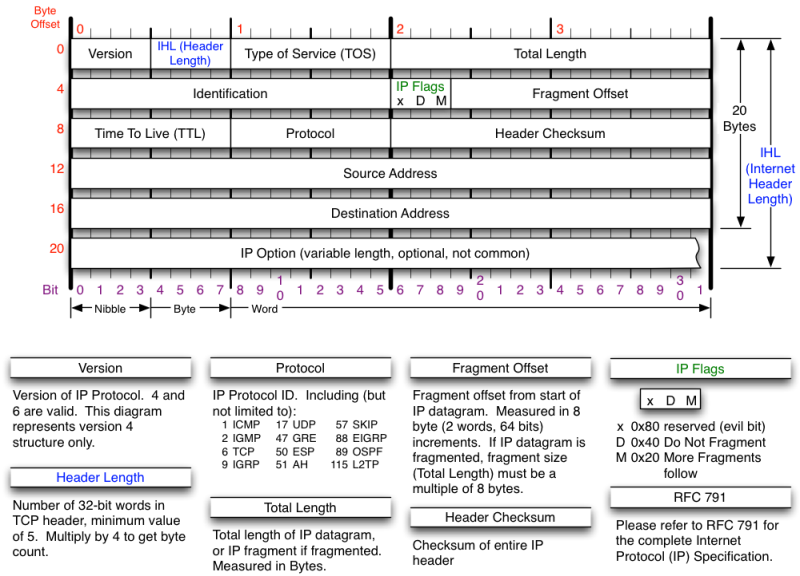
\includegraphics[scale=0.7]{images/IP-Header.png}\\[1cm]
\end{center}

\newpage







\section{CLEAN: Calculating, Legacy, Endianness, Addressing, Networks}

\subsection{Calculating: Counting}

\begin{description}
	\item[Counting] Process that starts with $n=0$ as the initial count. Every counted object is labeled with the actual $n$ value, and n is updated to $n=n+1$. Process ends when all objects have been counted.
\end{description}
	
	
\subsection{Legacy}

\begin{itemize}
	\item Everybody knows what Karst thinks of legacy.
\end{itemize}


\subsection{2-adic vs Binary}

\begin{center}
  \begin{tabular}{ | c | c | c | c | }
    2-adic & Binary & 2-adic to base-10 & Binary to base-10 \\ \hline
    1 & 0 & 1 & 0 \\ \hline
    2 & 1 & 2 & 1 \\ \hline
    11 & 00 & 3 & 0 \\ \hline
    12 & 01 & 4 & 1 \\ \hline
    21 & 10 & 5 & 2 \\ \hline
    22 & 11 & 6 & 3 \\ \hline
    111 & 000 & 7 & 0 \\ 
    \hline
  \end{tabular}
\end{center}

\begin{itemize}
	\item The whole point is that binary resets at every range increase.
\end{itemize}


\subsection{Big-endian and Little-endian}

\begin{center}
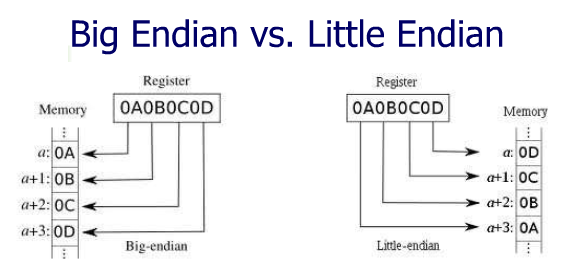
\includegraphics[scale=0.5]{images/BI-LI.png}\\[1cm]
\end{center}


\subsection{Addressing}

\begin{itemize}
	\item \url{http://www.exploringbinary.com/binary-converter/}
\end{itemize}


\newpage







\section{IPv6}


\subsection{Rationale}

\begin{itemize}
	\item $4x$ address space size increase $=$ $2^{96}$ address number increase.
	\item Headers have a fixed size of 40 bytes. Supports extended headers for additional functionality.
	\item NATs no longer needed due the vast amount of addresses.
\end{itemize}


\subsection{Addressing}

\begin{itemize}
	\item 128-bit addresses.
	\item 8 blocks of 4 nibbles ($8x4x4 = 128$ bits)
	\item Consecutive blocks of all-zeroes can be replaced by $::$ once.
	\item No broadcasts, no subnet masks.
	\item \url{http://www.iana.nl/assignments/ipv6-address-space/ipv6-address-space.xhtml}
\end{itemize}


\begin{description}
	\item[Reserved addresses]
\end{description}
	\begin{center}
	\begin{tabular}{ | c | c | }
		\hline
		::/8 & Special-purpose \\ \hline
		100::/8 & Special-purpose \\ \hline
		2000::/3 & Global unicast \\ \hline
		fc00::/7 & Unique local unicast \\ \hline
		fe80::/10 & Link-local (Link-scoped) unicast \\ \hline
		ff00::/8 & Multicast \\
		\hline
	\end{tabular}
	\end{center}

\begin{description}
	\item[Special-purpose addresses]
\end{description}
	\begin{center}
  	\begin{tabular}{ | c | c | }
    	\hline
		::/128 & Unspecified address \\ \hline
		::1/128 & Localhost address \\ \hline
		::a.b.c.d/128(from ::/96) & IPv4-compatible addresses \\ \hline
		::ffff:a.b.c.d/128 (from ::ffff:0:0/96) & IPv4-mapped addresses \\ \hline
		64:ff9b::/96 & Well-known prefix \\ \hline
		100::/64 & Discard-only address block \\
		\hline
	\end{tabular}
	\end{center}
	
	
\subsection{Neighbour Discovery Protocol (NDP)}
	
\begin{itemize}
	\item IPv6 does not use ARP. Uses ICMPv6 instead.
	\item ICMPv6 types for NDP:
\end{itemize}	

\begin{center}
  	\begin{tabular}{ | c | c | }
    	\hline
		133 & Router Solicitation \\ \hline
		134 & Router Advertisement \\ \hline
		135 & Neighbor Solicitation \\ \hline
		136 & Neighbor Advertisement \\ \hline
		137 & Redirect Message \\
		\hline
	\end{tabular}
\end{center}


\subsection{IPv6 Header}

\centerline{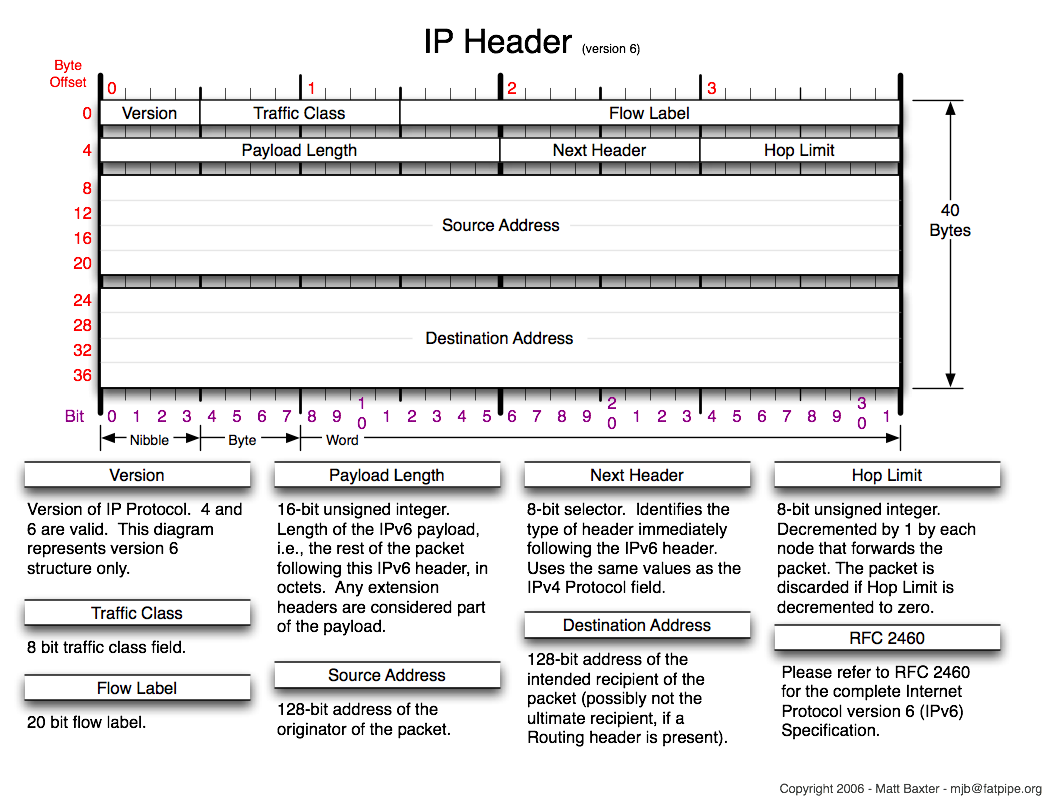
\includegraphics[scale=0.45]{images/IPv6-Header.png}\\[1cm]}


\newpage


\section{Layer 2: Bridging and Switching}

\subsection{Layers 1 and 2}

\begin{description}
	\item[Layer 1] Repeaters, hubs. Same collision domain. Same link segment.
	\item[Layer 2] Bridges, switches. Same collision domain. Same link segment.
\end{description}
	
	
\subsection{Layer 2: MAC and LLC}

\begin{description}
	\item[MAC] Media Access Control. Work from IEEE 802.3\footnote{\url{http://en.wikipedia.org/wiki/IEEE_802.3}}.
	\item[CSMA/CD] Carrier Sense Multiple Access With Collision Detection. Ethernet is the most common.
	\begin{enumerate}
    	\item Is my frame ready for transmission? If yes, move to 2.
    	\item Is medium idle? If not, wait until it becomes ready.
    	\item Start transmitting.
    	\item Did a collision occur? If so, go to collision detected procedure.
    	\item Reset retransmission counters and end frame transmission.
	\end{enumerate}
	\item[LLC] Logical Link Control. Multiplexing mechanisms, flow control and error management. Interface between MAC and Network Layer.
\end{description}
	
\subsection{Frame Formats}

\centerline{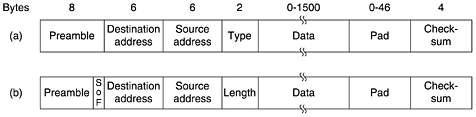
\includegraphics[scale=0.7]{images/Ethernet.png}\\[1cm]}

\begin{description}
	\item[DIX Ethernet] DEC-Intel-Xerox initial frame structure\footnote{\url{http://www.epubbud.com/read.php?g=5HEKFDZU&two=1&tocp=38}}.
	\begin{description}
    	\item[8bytes Preamble] Each one containing $10101010$. Used for synchronization.
    	\item[6bytes Destination Address]
    	\item[6bytes Source Address]
    	\item[2bytes Type] Indicator of the used transport protocol.
    	\item[0-1500bytes Payload]
    	\item[0-46bytes Pad] Valid Ethernet frames have, at least, 64 bytes (not counting Preamble!). If a frame is less than that (Payload < 46bytes), a pad is added to it. This is done to ease collision detection.
    	\item[4bytes Checksum] CRC of all the frame fields.
	\end{description}
	\item[802.3 Ethernet] Changes from DIX:
	\begin{description}
    	\item[7bytes Preamble + 1byte Start of Frame] Same as before but changing last byte to have compatibility with 802.4 and 802.5 (Token Bus and Token Ring).
    	\item[2bytes type -> 2bytes length] IEEE tried to change the purpose of the field (and move "type" information to *inside* the Payload), but some people did not change. Rule of thumb: if its value is over 1500, it is a Length field, otherwise it is a Type field.
    	\item[Changes on the Payload] There are 8 additional bytes of 'metadata' on the payload that are used mostly for nothing, effectively reducing the MTU from 1500 to 1492.
	\end{description}
	
\end{description}


\subsection{MAC Addresses}

\begin{description}
	\item[MAC48] Physical, obsolete.
	\item[EUI48] Virtual, including physical.
	\item[EUI64] Extended.
	\item[OUI] First 24bits of the MAC address. Identify who issued the device.
\end{description}


\subsection{EUI48 to EUI64}

[0:23bits]:FF:FE:[24:--bits]. When used to generate IPv6 address, the 7th most significative bit is swapped.

\subsection{Ethernet Types}

\begin{description}
	\item[0x0800] IP
	\item[0x0806] ARP
	\item[0x86DD] IPv6
\end{description}

\subsection{Bridges and Switches}

\begin{description}
	\item[Transparent Bridges] Use Store-and-Forward. Copy data from one port to another (or multiple ports). They can learn (and remember) where other devices are when they receive messages.
	\item[Switches are synonyms of Bridges] Usually refer to bridges with multiple interfaces.
\end{description}

\subsection{VLANs (802.1Q-2011)}

\centerline{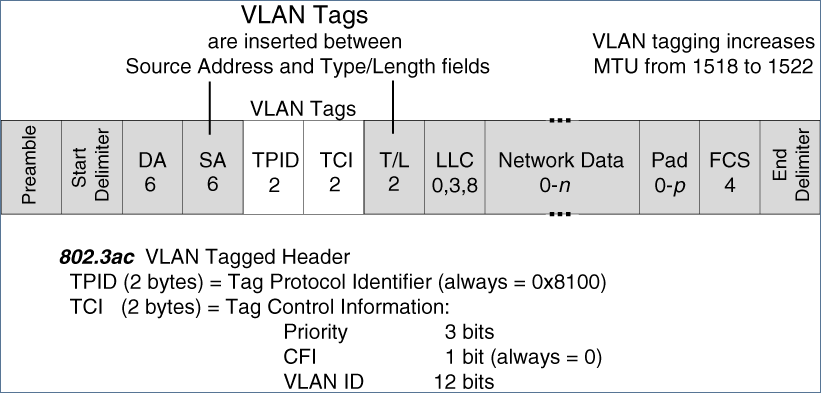
\includegraphics[scale=0.5]{images/VLAN.png}\\[1cm]}


\subsection{Layered Extensions}

TO-DO

\subsection{PBB-TE, TRILL, SPB}

TO-DO


\newpage









\section{STP Protocol}

\subsection{Goals and properties}

\begin{enumerate}
    \item Eliminate edges (connections) until there are no possible loops.
    \item After performing the algorithm, graph turns into a tree.
    \item Topology changes cause changes on the tree.
    \item Protocol works by electing a Root Node.
\end{enumerate}



\subsection{Configuration Messages}

\begin{description}
    \item[ID] based on a variable priority and its MAC address.
    \item[Root Node] Elected as the node with the lowest ID on the system.
    \item[Root ports on each Node] Chosen by\footnote{\url{https://www.youtube.com/watch?v=iB7BxtZVy3c}}:
    \begin{enumerate}
   		\item Lower advertised Root ID.
   		\item Lower advertised cost to Root.
   		\item Lower transmitting bridge ID.
   		\item Lower  port ID.
	\end{enumerate}
\end{description}

\centerline{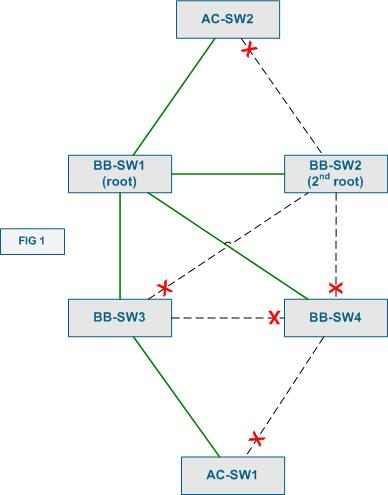
\includegraphics[scale=0.5]{images/STP-convergence.png}\\[1cm]}



\subsection{Timing Parameters}

\begin{description}
    \item[Hello Time] Time between two configuration messages.
    \item[Max Age] Parameter to discard messages that are too old.
    \item[Forward Delay] Half of the delay before transitioning from blocking to forwarding.
    \begin{enumerate}
   		\item Can be understood as two different waiting times. During that waiting, it does not forward packets.
   		\item First waiting: Listen for neighbours (other bridges).
   		\item Second waiting: Learn the location of MAC addresses.
	\end{enumerate}
\end{description}

\subsection{Topology Change Mechanism}


\begin{description}
   	\item[Memory] Bridges remember where other bridges are located.
   	\item[Stable Topology] When the topology is stable, bridges have a long caching time.
   	\item[Topology Changes] When a topology change is detected, the bridge detecting the change (and subsequent ones) sends a Topology Change Notification on his Root Port. When the message reaches the Root Bridge, it sets up its Topology Change flag. This causes other bridges to switch to the short caching delay.
\end{description}



\subsection{Bridge Protocol Data Unit (BPDU)}

\centerline{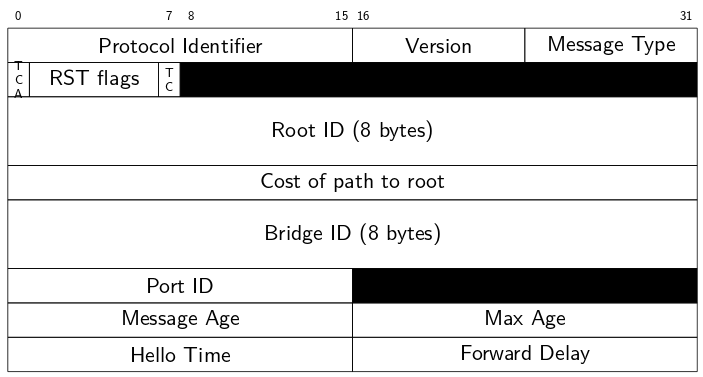
\includegraphics[scale=0.5]{images/BPDU.png}\\[1cm]}

\begin{description}
   	\item[Protocol Identifier] All zeroes.
   	\item[Version] 0 for STP, 2 for RST
   	\item[Message Type] 0 for Hello, 2 for RST, 128 for TCN
   	\item[Flags] TCA (Topology Change Ack), [Proposal, Agreement, ...], TC (Topology Change)
   	\item[Root ID]  Root Bridge.
   	\item[Cost to Root] Cost to the Root Bridge.
   	\item[Bridge ID] Bridge transmitting.
   	\item[Port ID] Port used on the transmitting bridge.
   	\item[Message Age] Age of the BPDU information.
   	\item[Max Age] Tipically 20 seconds (min 6).
   	\item[Hello Time] Tipically 2 seconds.
   	\item[Forward Delay] Tipically 15 seconds (min 4).
\end{description}

\subsection{STP Enhancements}

\begin{description}
   	\item[Rapid Spanning Tree (RST)] Changes on the BPDUs to make the algorithm faster.
   	\item[STP on VLANs] Global STP for all VLANs. Individual STP on each one of them.
   	\item[MSTP] Divide LAN into regions. Run STP on each one of them.
\end{description}




\newpage

\section{Routing}

\subsection{Basics}

\begin{description}
   	\item[Direct Routing] Added automatically by $ifconfig$ on unix systems.
   	\item[Global Routing] Done by using routing tables.
   	\item[Netstat/Route flags] Flags of the route command:
   	\begin{description}
   		\item[G] Needs gateway / directly connected.
   		\item[H] Route to Host / Route to Network
   		\item[S] Static route (manually added) / Dynamic route (added by a protocol)
	\end{description}
   	\item[ARP] Address Resolution Protocol.
   	\item[IP] Replacess $ifconfig$, $route$ and $arp$.
   	\item[Route Selection] Most specific entry on the routing table first. Use default if there is no match.
\end{description}




\subsection{Internet Routing}

\begin{description}
   	\item[Autonomous Systems (AS)] An AS is a connected group of one or more IP prefixes that has a single and well-defined routing policy. Each AS is managed by one or more operators and hosts a collection of routers and networks.
   	\item[Edge Routers] Edge Routers are used to communicate between different ASs, using an External Gateway Protocol such as BGP4 (which holds a monopoly in these type of communications).
   	\item[Internal Routers] Internal Routers use a different set of Internal Gateway Protocols (IGP) to communicate between themselves, such as RIP, OSPF or IS-IS.
\end{description}


\subsection{Dynamic Routing Mechanisms}

\begin{description}
   	\item[Distance Vector Routing (RIP)] Bellman-Ford.
   	\item[Link State Routing (OSPF)] Dijkstra
   	\item[Path Vector Routing (BGP)] 
\end{description}




\newpage

\section{Algorithms}



\subsection{Counting to Infinity Remarks}

\begin{enumerate}
   	\item In Computer Science, infinite is finite.
   	\item To avoid issues, do not advertise back to the advertiser (Split Horizon).
   	\item Poisoned Reverse: Announce back infinite cost to advertiser.
\end{enumerate}



\subsection{Bellman-Ford}

\centerline{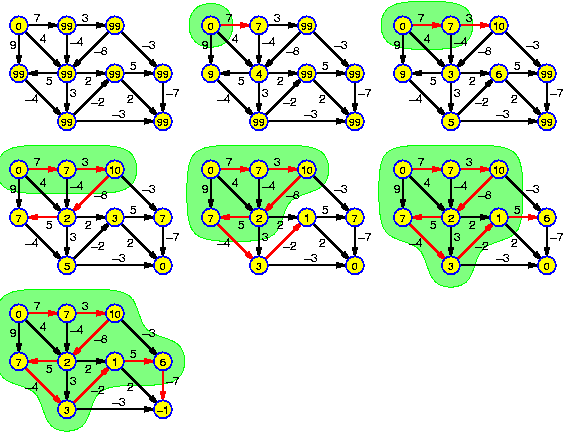
\includegraphics[scale=0.6]{images/bellman_ford.png}\\[1cm]}



\subsection{Shortest Path Tree (Dijkstra)}


\centerline{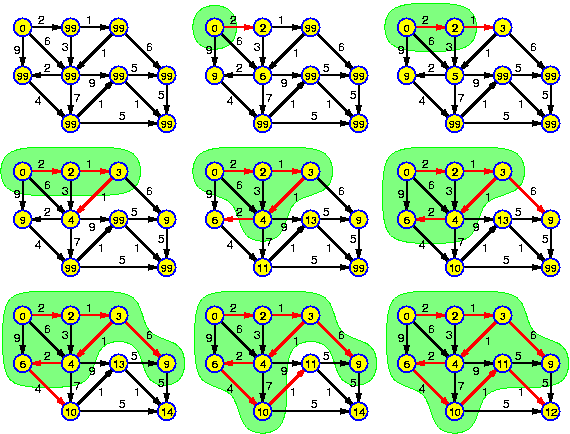
\includegraphics[scale=0.6]{images/dijkstra.png}\\[1cm]}



\subsection{Minimum Spanning Tree (Prim, Kruskal)}

\begin{description}
   	\item[Prim] Algorithm\footnote{\url{https://www.youtube.com/watch?v=cplfcGZmX7I}}:
   	\begin{enumerate}
   		\item Pick random node $N$ and add it to the tree $T$.
   		\item From all the vertex on the current tree $T$, pick $V_{i}$ with the lowest cost. Add the connected node to the tree.
   		\item Repeat 2 until all nodes are present on the tree.
	\end{enumerate}
   	\item[Kruskal] Algorithm\footnote{\url{https://www.youtube.com/watch?v=71UQH7Pr9kU}}:
   	\begin{enumerate}
   		\item Pick the lowest vertex on the graph and create a tree with the two nodes connected.
   		\item From the rest of the graph, pick the vertex with the lowest value that does not generate a loop. This will create new trees or expand the current ones.
   		\item Repeat 2 until all nodes are present on a single.
	\end{enumerate}
\end{description}



\newpage




\section{Distance Vector Protocol- RIP}



\subsection{RIP Version 1}

\subsubsection{Basics}

\begin{enumerate}
	\item Based on the Bellman-Ford algorithm.
	\item Keep a table of the routes to destinations as {distance (metric), gateway (next hop)}.
	\item Periodically send table to neighbours.
	\item Update table with incoming information (regularly can only get better, unless TC announced by root).
	\item Sent updates as soon as a route changes (later addition).
	\item Supports one level depth subnet masks. It differentiates updates from the same and another. networks.
	\item Infinity = 16 hops.
\end{enumerate}
	
\subsubsection{Timers}
	
\begin{description}
	\item[Update timer] updates are sent every 30 seconds.
	\item[Invalid/Timeout timer] routes time out after 180 seconds.
	\item[Flush timer] routes disappear after 240 seconds.
	\item[Hold-down timer] Prevent incorporating possibly bad routing information
which might be present in a network that didn’t converge yet (180 seconds).
\end{description}

\subsubsection{Packet Format}

\centerline{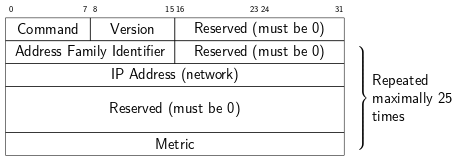
\includegraphics[scale=0.6]{images/RIPv1.png}\\[1cm]}

\begin{enumerate}
	\item Requests broadcasted to $255.255.255.255$ or to a directed broadcast address. Answers as unicast.
	\item Uses UPD port 520.
	\item UDP packet 512 bytes - 8 bytes UDP header: 504 bytes. 20 bytes/route = max 25 route updates/packet.
\end{enumerate}


\subsection{Protocol Extensions}


\subsubsection{Interior Gateway Routing Protocol (IGRP)}

\begin{enumerate}
	\item Runs directly on top of IP (protocol 9).
	\item Larger notion of infinity (100-255).
	\item Can handle up to four parallel paths.
	\item Uses three types of network routes.
	\item Metric includes, besides hop count, other information {delay, bandwidth, reliability and load}.
\end{enumerate}





\subsubsection{Enhanced Interior Gateway Routing Protocol (EIGRP)}

\begin{enumerate}
	\item Runs directly on top of IP (protocol 88).
	\item Keeps state of neighbours.
	\item Remembers $all$ paths.
\end{enumerate}

\subsection{RIP Version 2}


\centerline{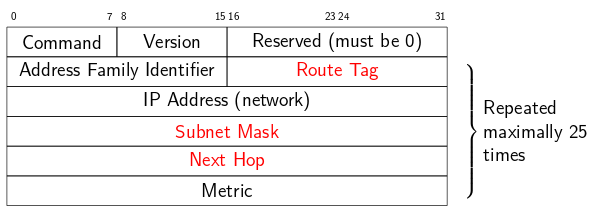
\includegraphics[scale=0.5]{images/RIPv2.png}\\[1cm]}

\begin{description}
	\item[Route Tag] Identification of route origin. Differentiates internally and externally generated routes. Can be used for authentication.
	\item[IP Address] Destination Network. RIPv2 uses multicast group 224.0.0.9, not broadcast.
	\item[Subnet Mask] CIDR support.
	\item[Next Hop] Gateway (if different from advertising router).
\end{description}



\subsection{RIPng}


\centerline{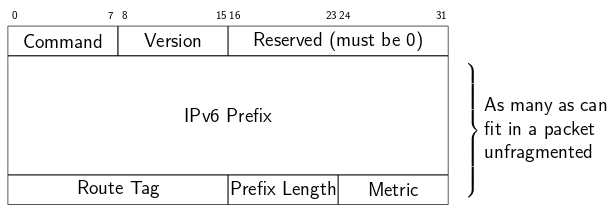
\includegraphics[scale=0.5]{images/RIPng.png}\\[1cm]}


\begin{enumerate}
	\item Runs on UPD (Port 521).
	\item Packets can be as large as MTU.
	\item Used in IPv6. Multicast address FF02::9.
\end{enumerate}






\newpage



\section{Link State Routing - OSPF}


\subsection{Basics}


\begin{enumerate}
	\item Based on the Dijkstra algorithm.
	\item Used instead of distance vector algorithms on more complex topologies.
	\item Faster convergence time than distance vector algorithms.
\end{enumerate}


\subsection{Link State Packets}

\begin{enumerate}
	\item LSP represent the state of a Router and its links to the rest of the network.
	\item Enough for point-to-point links.
	\item Broadcast Networks and NBMA networks are represented by virtual nodes.
\end{enumerate}

\subsection{Non-broadcast Networks}

\begin{description}
	\item[NBMA] Non-Broadcast Multiple Access
	\begin{enumerate}
		\item Full-mesh connectivity, but not permanently.
		\item Connectivity by Designated Routers (DR).
	\end{enumerate}
	\item[Point-to-multipoint]
	\begin{enumerate}
		\item Subset of all point-to-point links.
		\item No full-mesh.
		\item No DR elected.
	\end{enumerate}

\end{description}


\subsection{LSP Generation}

\begin{enumerate}
	\item Announcements every 30 minutes (RIP was 30 seconds)
	\item Announcements trigger as soon as changes are detected (link up/down, change on link cost).
	\item Use smart flooding to detect duplicates (propagation looks like a tree).
\end{enumerate}


\subsection{LSP Problems}

\begin{description}
	\item[LSP arriving out of order] Solutions: Timestamps and Sequence numbers. Timestamps require clock synchronization. Sequence numbers must be large enough to guarantee ordering, and the value should always be increased when forwarding the LSP. 
\end{description}
	
	
\subsection{OSPF Properties}
	
\begin{enumerate}
	\item Supports hierarchical routing and subnets.
	\item Efficient multicast for flooding.
	\item Uses metrics based on cost on each interface.
	\item Supports virtual links, load balancing, unnumbered interfaces and authentication.
	\item Built on top of IP (protocol 89).
	\item LSP are named LSA (Link State Advertisement).
	\item OSPF uses multicast address 224.0.0.6 (FF02::6) for DR and multicast address 224.0.0.5 (FF02::5) for all routers.
\end{enumerate}


\subsection{Parameters and LSAs}
	
\begin{enumerate}
	\item Timing parameters must be the same for all OSPF neighbours.
	\item If routing table overflows, external routers are dropped first to generate space.
	\item LSAs must be acknowledged, and can be queued for transmission. They must time out at about the same time.
\end{enumerate}





\subsection{Network representation}
	
\begin{enumerate}
	\item A DR and a Backup Designated Router (BDR) are elected on each multi-access network with Hello packets. The (B)DR represents the network as a virtual node and acts on its behalf. Routers can have custom priorities for the election.
	\item Hierarchical Routing:
\end{enumerate}


\centerline{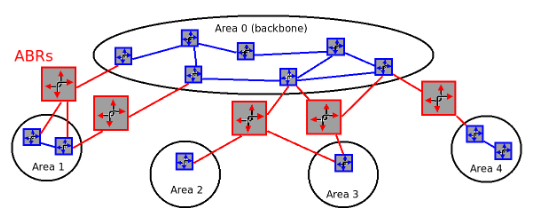
\includegraphics[scale=0.5]{images/OSPF.png}\\[1cm]}


\subsection{Router Types}
	
\begin{description}
	\item[Backbone Router] At least one interface is inside in the Backbone (Area 0).
	\item[Internal Router] All interfaces are in the same Area.
	\item[Area Border Router (ABR)] Has one interface in the Backbone and one or more in other areas.
	\item[Autonomous System Boundary Router (ASBR)] Participates in external routing protocols.
\end{description}



\subsection{Stubby Areas}
	
\begin{description}
	\item[Stubby Area] Area in which no external routing information is injected by the ABRs.
	\item[Totally Stubby Area] Stubby Area in which not even inter-area summaries are injected.
	\item[Not-So-Stubby Area]  Stubby Area in which external routing information can be generated and propagated locally.
\end{description}



\subsection{OSPF Packet Format}
	

\centerline{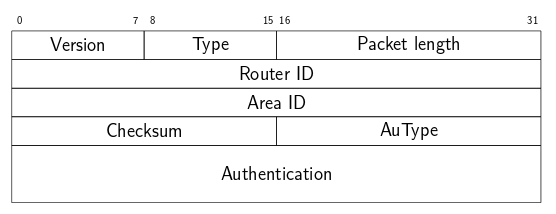
\includegraphics[scale=0.5]{images/OSPFformat.png}\\[1cm]}

\begin{description}
	\item[Type 1: Hello Packet] Sent periodically to 224.0.0.5 multicast address on all interfaces (unicast on virtual-links), enabling dynamic discovery and refresh of neighbors. On broadcast and NBMA networks, Hello packets are used to elect DR and BDR\footnote{\url{https://sites.google.com/site/amitsciscozone/home/important-tips/ospf/ospf-packet-types}}.
	\item[Type 2: Database Description] The OSPF router summarizes the local database and the DBD packets carry a set of LSAs belonging to the database. When a neighbor sees an LSA that is more recent than its own database copy, it requests this newer LSA from the neighbor.
	\item[Type 3: Link State Request] After DBD packets exchange process, the router may find it does not have an up-to-date database. The LSR packet is used to request pieces of neighbor database that is more up-to-date. 
	\item[Type 4: Link State Update] These packets implement the flooding of LSAs. Each LSA contains routing, metric and topology information to describe a portion of OSPF network.
	\item[Type 5: Link State Acknowledgement] OSPF requires acknowledgment for the receipt of each LSA. Multiple LSAs can be acknowledged in a single LSAck packet.
\end{description}

\subsection{OSPFv3}

TO-DO


\newpage

\section{Path Vector Routing - BGP}

\subsection{Basics of BGP(4)}


\begin{enumerate}
	\item Inter-AS protocol monopoly.
	\item Based on Path-Vector Routing.
	\item ASs have a custom defined set of policies for routing.
	\item BGP works on TCP port 179.
	\item Exchanges Network Layer Reachability Information (NLRI)
\end{enumerate}


\subsection{Routing Policies: Customers, Peers and Providers}


\begin{description}
	\item[Customers] Highest preference.
	\item[Peers] Next highest preference. If peers are similar, usually money transactions are neglected.
	\item[Providers] Lowest preference. 
\end{description}

\begin{description}
	\item[Advertising Customers] All routes are advertised to customers, and routes to customers are advertised to other Peers and Providers.
	\item[Advertising Peers and Providers] Peer and Provider routes are not advertised to other Peers or Providers.
\end{description}


\subsection{External BGP (EBGP) and Internal BGP (IBGP}

\begin{description}
	\item[EBGP (between ASs)] Exchange prefixes and implementing policies.
	\item[IBGP (within one AS)] Create a consistent view of all entry/exit points. IBGP routes are not distributed to other IBGPs to prevent loops. 
\end{description}


\subsection{BGP Information Bases}


\begin{description}
	\item[Adj-RIB-In] One per peer. Routes after input filtering.
	\item[Loc-RIB] Only one globally. Routes after best path selection.
	\item[Adj-RIB-Out] One per peer. Routes after output filtering.
\end{description}


\subsection{BGP Attributes}

In order of path selection preference:

\begin{description}
	\item[LOCAL-PREF] Advertised within a local AS. Used for local policies. Default value is 100, highest value wins.
	\item[AS-PATH] Sequence of ASs. Can be used for loop detection, and the sequence length measures the metric. Own AS can be prepended multiple times in EBGP for traffic engineering. This does not consider path length inside a certain AS.
	\item[ORIGIN] States where the route did origin (NLRI)
	\item[MULTI-EXIT-DISC] Advertised between neighbour ASs via EBGP, and not transferred to third ASs. Lower MED wins.
\end{description}

\centerline{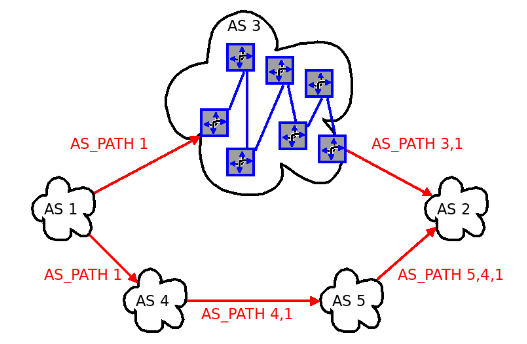
\includegraphics[scale=0.5]{images/AS_PATH.png}\\[1cm]}



Unrelated to path selection:

\begin{description}
	\item[NEXT-HOP] Must be reachable unless in case of multi-hop BGP.
\end{description}



\centerline{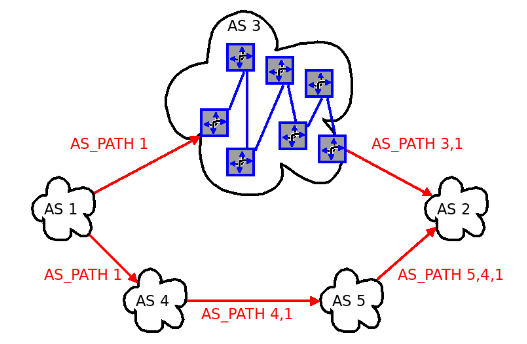
\includegraphics[scale=0.5]{images/AS_PATH.png}\\[1cm]}
	
	

\subsection{BGP Messages (not packets!)}	


\begin{description}
	\item[OPEN] Establish a peering session. Includes information such as BGP version, AS number, and IP address.
	\item[UPDATE] Announcing new information: new rules and deleted rules.
	\item[NOTIFICATION] Error notification.
	\item[KEEP-ALIVE] Blank packet at regular intervals.
	\item[REFRESH] Ask peer for a refresh of its information.
\end{description}


\subsection{Traffic Engineering}	

\begin{description}
	\item[Outbound Traffic] AS is in charge of this engineering. Attributes can be tweaked to select most suitable routes. Usually done by changing local preference.
	\item[Inbound Traffic] AS depends on other's ASs policies for this. Attributes can be tweaked to attempt to influence other peer's decisions. Can be done (kinda of a "hack") by extending outbound AS-PATH or by manipulating the MED\footnote{\url{http://www.cisco.com/c/en/us/support/docs/ip/border-gateway-protocol-bgp/112965-bgpmed-attr-00.html}}. However best approach is to contact other ASs administrators and reach an agreement (use of "communities" for automation).
\end{description}



\subsection{IBGP Scaling}	

\begin{description}
	\item[Route Reflectors] A big IBGP peer, using full-mesh connectivity.
	\item[Confederations] Use subASs inside your AS, hiding their existence to the outside world.
\end{description}
	
\newpage


\printbibliography

\end{document}
